\documentclass{article}

% latex math commands
% Vladimir Feinberg
% \vx notation for vectors from Goodfellow
% https://github.com/goodfeli/dlbook_exercises

% alphabet templates
% abcdefghijklmnopqrstuvwxyz
% ABCDEFGHIJKLMNOPQRSTUVWXYZ

% fonts, math, and layout commands
\usepackage{lmodern}
\usepackage{fullpage}
\usepackage{bbm}
\usepackage{enumerate}
\usepackage{amsmath}
\usepackage{amsthm}
\usepackage{amssymb}
\usepackage{amsfonts}
\usepackage{mathrsfs}
\usepackage{mathtools}
\usepackage[all]{xy}
\usepackage{algorithm}
\usepackage[noend]{algpseudocode}

% include graphics with \includegraphics
\usepackage{graphicx}
\usepackage{caption}

% \nicefrac{x}{y} gives a diagonal fraction bar x/y
\usepackage{nicefrac}

% \nurl{<url>}{link name} renders a blue underlined link
\usepackage[hidelinks]{hyperref}
\usepackage{xcolor}
\usepackage{url}
\newcommand{\nurl}[2]{\href{ #1 }{\color{blue}\underline{#2}}}

% brackets, norms, cardinalities
\newcommand{\pa}[1]{ \left({#1}\right) }
\newcommand{\ha}[1]{ \left[{#1}\right] }
\newcommand{\ca}[1]{ \left\{{#1}\right\} }
\newcommand{\inner}[1]{\left\langle #1 \right\rangle}
\newcommand{\innercpy}[1]{\inner{ #1, #1 }}
\newcommand{\norm}[1]{\left\lVert #1 \right\rVert}
\newcommand{\card}[1]{\left\lvert{#1}\right\rvert}
\newcommand{\abs}[1]{\card{#1}}

% math vectors
\newcommand{\va}{\textbf{a}}
\newcommand{\vb}{\textbf{b}}
\newcommand{\vc}{\textbf{c}}
\newcommand{\vd}{\textbf{d}}
\newcommand{\ve}{\textbf{e}}
\newcommand{\vf}{\textbf{f}}
\newcommand{\vg}{\textbf{g}}
\newcommand{\vh}{\textbf{h}}
\newcommand{\vi}{\textbf{i}}
\newcommand{\vj}{\textbf{j}}
\newcommand{\vk}{\textbf{k}}
\newcommand{\vl}{\textbf{l}}
\newcommand{\vm}{\textbf{m}}
\newcommand{\vn}{\textbf{n}}
\newcommand{\vo}{\textbf{o}}
\newcommand{\vp}{\textbf{p}}
\newcommand{\vq}{\textbf{q}}
\newcommand{\vr}{\textbf{r}}
\newcommand{\vs}{\textbf{s}}
\newcommand{\vt}{\textbf{t}}
\newcommand{\vu}{\textbf{u}}
\newcommand{\vv}{\textbf{v}}
\newcommand{\vw}{\textbf{w}}
\newcommand{\vx}{\textbf{x}}
\newcommand{\vy}{\textbf{y}}
\newcommand{\vz}{\textbf{z}}
\newcommand{\vzero}{\textbf{0}}
\newcommand{\vone}{\textbf{1}} 
\newcommand{\valpha}{{\boldsymbol\alpha}}
\newcommand{\vepsilon}{{\boldsymbol\epsilon}}
\newcommand{\veta}{{\boldsymbol\eta}}
\newcommand{\vsigma}{ {\boldsymbol\sigma}}
\newcommand{\vtheta}{ {\boldsymbol\theta}}
\newcommand{\vdelta}{ {\boldsymbol\delta}}
\newcommand{\vlambda}{ {\boldsymbol\lambda}}
\newcommand{\vmu}{ {\boldsymbol\mu}}
\newcommand{\vvartheta}{ {\boldsymbol\vartheta}}
\newcommand{\vbeta}{ {\boldsymbol\beta}}
\newcommand{\vphi}{ {\boldsymbol\phi}}


% math function arrows, misc binary math ops
\newcommand{\bij}{\leftrightarrow}
\newcommand{\inj}{\rightarrowtail}
\newcommand{\sur}{\twoheadedrightarrow}
\newcommand{\eqd}{\mathrel{\overset{\Delta}{=}}}

% common math sets
\newcommand{\Z}{\mathbb{Z}}
\newcommand{\R}{\mathbb{R}}
\newcommand{\C}{\mathbb{C}}
\newcommand{\N}{\mathbb{N}}
\newcommand{\Q}{\mathbb{Q}}
\newcommand{\F}{\mathbb{F}}
\newcommand{\T}{\mathbb{T}}

% limits
\def\sumn{\sum_{n=0}^\infty}
\def\limn{\lim_{n\rightarrow\infty}}
\def\prodn{\prod_{n=0}^\infty}

% mathcal
\newcommand{\mcA}{\mathcal{A}}
\newcommand{\mcB}{\mathcal{B}}
\newcommand{\mcC}{\mathcal{C}}
\newcommand{\mcD}{\mathcal{D}}
\newcommand{\mcE}{\mathcal{E}}
\newcommand{\mcF}{\mathcal{F}}
\newcommand{\mcG}{\mathcal{G}}
\newcommand{\mcH}{\mathcal{H}}
\newcommand{\mcI}{\mathcal{I}}
\newcommand{\mcJ}{\mathcal{J}}
\newcommand{\mcK}{\mathcal{K}}
\newcommand{\mcL}{\mathcal{L}}
\newcommand{\mcM}{\mathcal{M}}
\newcommand{\mcN}{\mathcal{N}}
\newcommand{\mcO}{\mathcal{O}}
\newcommand{\mcP}{\mathcal{P}}
\newcommand{\mcQ}{\mathcal{Q}}
\newcommand{\mcR}{\mathcal{R}}
\newcommand{\mcS}{\mathcal{S}}
\newcommand{\mcT}{\mathcal{T}}
\newcommand{\mcU}{\mathcal{U}}
\newcommand{\mcV}{\mathcal{V}}
\newcommand{\mcW}{\mathcal{W}}
\newcommand{\mcX}{\mathcal{X}}
\newcommand{\mcY}{\mathcal{Y}}
\newcommand{\mcZ}{\mathcal{Z}}

% measure theory
\newcommand{\indicator}{\mathbbm{1}}
\DeclareMathOperator{\Laplace}{Laplace}
\DeclareMathOperator{\Poisson}{Poisson}
\DeclareMathOperator{\Exponential}{Exponential}
\DeclareMathOperator{\Multinomial}{Multinomial}
\DeclareMathOperator{\Bernoulli}{Bernoulli}
\DeclareMathOperator{\Categorical}{Categorical}
\DeclareMathOperator{\Uniform}{Uniform}
\DeclareMathOperator{\Binomial}{Binomial}
\DeclareMathOperator{\Hypergeometric}{Hypergeometric}
\DeclareMathOperator{\GammaDist}{Gamma}
\DeclareMathOperator{\NegativeBinomial}{NegativeBinomial}
\DeclareMathOperator\mathProb{\mathbb{P}}
\renewcommand{\d}[1]{\mathop{\mathrm{d} #1 }}
\DeclarePairedDelimiterX{\infdivx}[2]{(}{)}{ #1\;\delimsize\|\;#2 }
\newcommand{\dkl}[2]{\mathop{D_\text{KL}}\infdivx{#1}{#2}}

% distributions
\makeatletter
\newcommand{\distas}[1]{\mathbin{\overset{#1}{\kern\z@\sim}}}%
\makeatother
\newcommand{\disteq}{\overset{d}{=}}
\newcommand{\distiid}{\distas{\text{iid}}}
\newcommand\independent{\protect\mathpalette{\protect\independenT}{\perp}}
\def\independenT#1#2{\mathrel{\rlap{$#1#2$}\mkern2mu{#1#2}}}
\newcommand{\convdist}{\mathbin{\overset{\text{d}}{\longrightarrow}}}
\newcommand{\convas}{\mathbin{\overset{\text{as}}{\longrightarrow}}}
\newcommand{\convpb}{\mathbin{\overset{\text{pb}}{\longrightarrow}}}

\renewcommand{\P}{\mathProb} % need to overwrite stupid paragraph symbol
\DeclareMathOperator\mathExp{\mathbb{E}}
\DeclareMathOperator*\mathExpUnder{\mathbb{E}}
\newcommand{\E}{\mathExp}

\newcommand{\sa}{{$\sigma$-algebra}}
\newcommand{\OR}{{\overline{\R}}}
\newcommand{\OX}{{\overline{X}}}
\DeclareMathOperator{\power}{{\mathcal{P}}}
\DeclareMathOperator{\var}{var}
\DeclareMathOperator{\cov}{cov}

% \set{from set}{condition} with set-builder notation
% conditional expectation is analogous
\newcommand{\set}[2]{ \left\{ #1 \,\middle|\, #2 \right\} }
\newcommand{\CE}[2]{ \mathExp\left[ #1 \,\middle|\, #2 \right] }

% linear-algebra related
\newcommand{\mat}[1]{\begin{pmatrix} #1 \end{pmatrix}}
\newcommand{\detmat}[1]{\begin{vmatrix} #1 \end{vmatrix}}
\DeclareMathOperator{\spanb}{span}
\DeclareMathOperator{\conv}{conv} % convex hull
\DeclareMathOperator{\cone}{cone}
\DeclareMathOperator{\vectorize}{vec}
\DeclareMathOperator{\matricize}{mat}
\DeclareMathOperator{\adj}{adj}
\DeclareMathOperator{\diag}{diag}
\DeclareMathOperator{\tr}{tr}
\DeclareMathOperator{\rank}{rank}
\DeclareMathOperator*{\argmin}{argmin}
\DeclareMathOperator*{\argmax}{argmax}
\DeclareMathOperator*{\proj}{proj}

% complex analysis
\DeclareMathOperator{\MyRe}{Re}
\DeclareMathOperator{\MyIm}{Im}
\DeclareMathOperator{\image}{image}
\DeclareMathOperator{\supp}{supp}

% typical numerical operators
\DeclareMathOperator{\sgn}{sgn}

% graphs
\DeclareMathOperator{\diam}{diam}

% constants
\renewcommand{\d}[1]{\mathop{\mathrm{d} #1 }}
\newcommand{\e}{\mathrm{e}}
\renewcommand{\i}{\imath}

% \bigtimes: large indexed cross product
\makeatletter
\DeclareFontFamily{U}  {MnSymbolF}{}
\DeclareSymbolFont{symbolsMN}{U}{MnSymbolF}{m}{n}
\SetSymbolFont{symbolsMN}{bold}{U}{MnSymbolF}{b}{n}
\DeclareFontShape{U}{MnSymbolF}{m}{n}{
    <-6>  MnSymbolF5
   <6-7>  MnSymbolF6
   <7-8>  MnSymbolF7
   <8-9>  MnSymbolF8
   <9-10> MnSymbolF9
  <10-12> MnSymbolF10
  <12->   MnSymbolF12}{}
\DeclareFontShape{U}{MnSymbolF}{b}{n}{
    <-6>  MnSymbolF-Bold5
   <6-7>  MnSymbolF-Bold6
   <7-8>  MnSymbolF-Bold7
   <8-9>  MnSymbolF-Bold8
   <9-10> MnSymbolF-Bold9
  <10-12> MnSymbolF-Bold10
  <12->   MnSymbolF-Bold12}{}
\DeclareMathSymbol{\tbigtimes}{\mathop}{symbolsMN}{2}
\newcommand*{\bigtimes}{%
  \DOTSB
  \tbigtimes
  \slimits@ 
}
\makeatother

% category theory arguments
% See https://tex.stackexchange.com/questions/356873
\newcommand{\catfst}{{-}}
\newcommand{\catsnd}{{=}}
\newcommand{\cattrd}{{\equiv}}
\DeclareMathOperator{\Id}{Id}
\newcommand{\opcat}[1]{{#1}^{\text{op}}}
\DeclareMathOperator{\Hom}{hom}
\DeclareMathOperator{\Ob}{ob}
\DeclareMathOperator{\El}{el}
\DeclareMathOperator{\colim}{colim}
\DeclareMathOperator{\Sym}{Sym}

% references
\newcommand{\figref}[1]{Figure~\ref{fig:#1}}
\newcommand{\tabref}[1]{Table~\ref{tab:#1}}
\newcommand{\secref}[1]{Section~\ref{sec:#1}}
\newcommand{\equref}[1]{Equation~\ref{eq:#1}}
\renewcommand{\algref}[1]{Algorithm~\ref{alg:#1}}

% centered figure with \autofig{filepath}{\label{fig:somelabel}}{caption}
\newcommand{\autofig}[3]{
  \begin{figure}[!ht]
    \begin{center}
      \includegraphics[width=0.8\columnwidth]{#1}
    \end{center}
    \caption{#3}
    #2
\end{figure}
}

\usepackage{fancyvrb}
\usepackage{verbatimbox}
\usepackage{placeins}
\title{Model-based RL Report\\\large CS 294-112}
\author{Vladimir Feinberg}
\date{10 October 2017}

\begin{document}
	
\maketitle

\section{Main Assignment}

In this assignment, I implemented model-based RL through an MPC controller. In particular, we consider learning the dynamics for the \texttt{HalfCheetah-v1} environment and using those dynamics to simulate rollouts with random actions, taking the action that resulted in the lowest cost after the simulation. The cost function is manually specified for the task. All invocations are available in the \texttt{README.md} file in the submitted assignment code.

Unless otherwise specified, all parameters are their defaults: 5 different seeds for each setup, 60 epochs of dynamics training on the full dataset per on-policy iteration, a dynamics batch size of 512, maximum episode length of 1000, 1000 simulated paths in the MPC controller, and 10 paths sampled by the initial random agent and then by the MPC controller that are aggregated every policy iteration. The learning rate was the default $10^{-3}$.

Even after learning dynamics from a random sample, the MPC controller performs fairly well (without any aggregated on-policy iterations) (Fig.~\ref{fig:oneit}).

\verbfilebox{iter-output.tex}
\begin{figure}[!h]
  \begin{center}
\theverbbox
  \end{center}
  \caption{MPC controller performance without any aggregated data.}
\label{fig:oneit}
\end{figure}

\FloatBarrier

Next, we evaluate whether we're actually learning the dynamics (Fig.~\ref{fig:learn-dyn}). We note that MSE is generally low, but actually improves in the aggregating case because of the extra training data improving generalization.

\begin{figure}[!h]
  \begin{center}
    {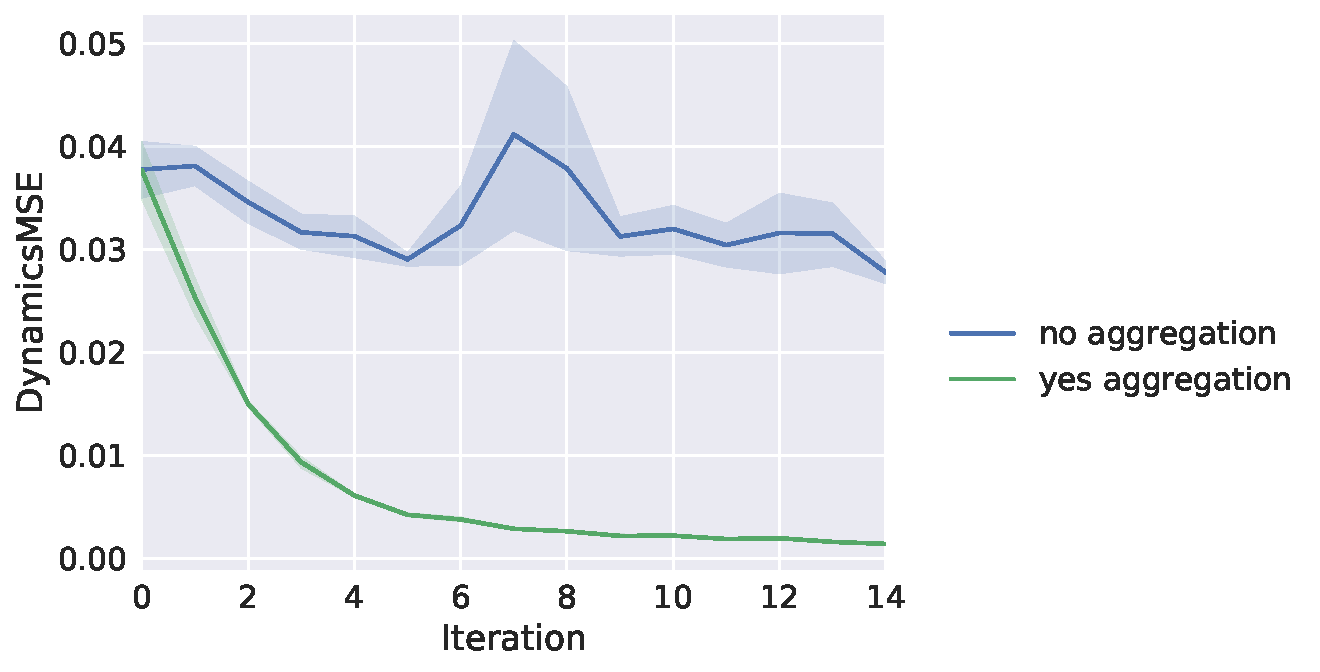
\includegraphics[width=0.8\textwidth]{DynamicsMSE.pdf}}
  \end{center}
  \caption{Unnormalized next-state prediction MSE over several iterations of 60-epoch rounds of full-dataset training. We show learning performance with data aggregation (i.e., a changing optimization target for optimization) and without data aggregation (the simpler problem of only learning only the first round of randomly-sampled policy transitions. Note that the MSE metric here is collected from a random agent sampled on unseen, newly reset environments (in the aggregation, this validation data is added into the training set after validating it).}
\label{fig:learn-dyn}
\end{figure}

\FloatBarrier

Finally, we evaluate the effect of including on-policy aggregated data from the randomly-sampling MPC controller (Fig.~\ref{fig:agg-returns}).

\begin{figure}[!h]
  \begin{center}
    {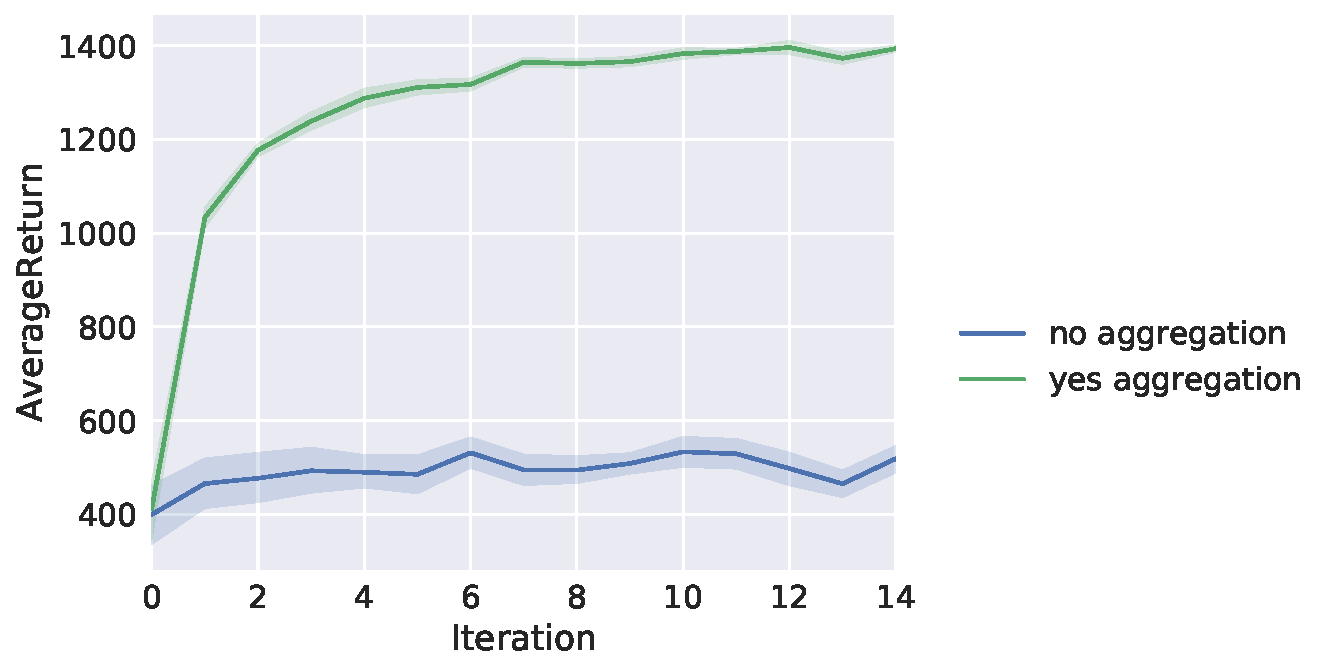
\includegraphics[width=0.8\textwidth]{AverageReturn.pdf}}
  \end{center}
  \caption{Comparison of average returns with and without on-policy aggregation for the randomly-sampling MPC controller. We compare over 15 such on-policy iterations with 10 sampled on-policy paths each, and display statistics only from the most recent sample. In the case of no aggregation, different iterations reflect samples of the performance of an MPC controller with a dynamics model iteratively learning from the same initial randomly-sampled set of transitions.}
\label{fig:agg-returns}
\end{figure}

\begin{figure}[!h]
  \begin{center}
    {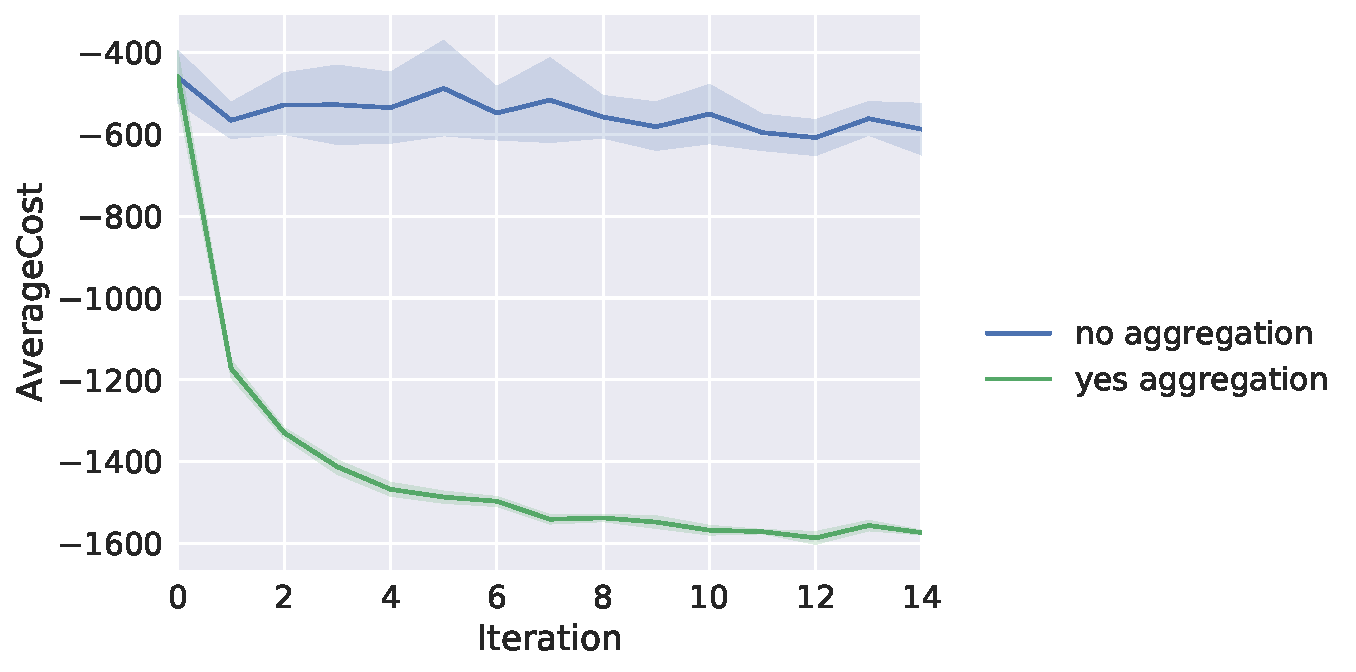
\includegraphics[width=0.8\textwidth]{AverageCost.pdf}}  
  \end{center}
  \caption{Comparison of average costs with and without on-policy aggregation for the randomly-sampling MPC controller in the same setting as Fig.~\ref{fig:agg-returns}.}
\label{fig:agg-costs}
\end{figure}

\FloatBarrier

\section{Extension: Speed}

To enable rapid development, I implemented several optimizations for the MPC controller. After following all of these in succession, I was able to get a single MPC iteration (i.e., with all default flags, 10 MPC rollouts total) speed \textbf{down to ${\mathbf{104.11
}}$ seconds}, compared to \textbf{around 600 seconds} in a vanilla implementation (only batching within the MPC controller). These results are on an Nvidia K20 GPU.
\begin{enumerate}
\item (Vanilla) assuming the MPC controller expands $p$ simulation paths, batch the dynamics prediction in these $p$ simulated rollouts for each time step that is simulated (for a horizon $h$ of simulated timesteps). At this point, the GPU is about 10\% utilized.
\item When sampling $i$ (non-simulated) rollouts total from the MPC controller, use $i$ independently-seeded environments and request actions from the MPC controller for all $i$ states in each of the environments simultaneously. Within the MPC controller, batch the dynamics prediction to $ip$ simultaneous predictions for each of $h$ time steps simulated. At this point, the GPU is about 50\% utilized.
\item Push the MPC loop onto the GPU alone by using a \texttt{tf.while\char`_loop} for the MPC rollout. This requires coupling the dynamics computation graph with the MPC one so the entire MPC rollout can stay within GPU memory in one \texttt{tf.Session.run} call (this would also be wayyy easier in PyTorch). This is by far the biggest speedup, now at about 85\% GPU utilization.
\item Eke out the last bit of performance by pushing trajectory cost function evaluation into the MPC controller loop. This is a win since the cost is additive across states so the GPU no longer needs to keep track of the entire rollout state matrix. This hits about 90\% utilization.
\end{enumerate}

\section{Extension: No Delta Normalization}

The assignment specification requires training the dynamics model $f$ on normalized outputs (where learned outputs are the changes to the dynamics, $f(\hat{s})\approx \hat{\delta}$, with $\hat{\cdot}$ indicating normalized values and $\delta=s'-s$ being the state transition). This requires learning statistics for state transition differences $\delta$.

This seemed a bit unstable to me, since some dimensions of $\delta$ might reasonably be concentrated around 0 for most transitions. For this reason, I considered predicting the difference in normalized states alone $\hat{s'}-\hat{s}$, which is still invariant to state distribution location and scale. Its performance with the regular $\delta$-normalizing approach is explored (Fig.~\ref{fig:deltanorm}).

\begin{figure}[!h]
  \begin{center}
    {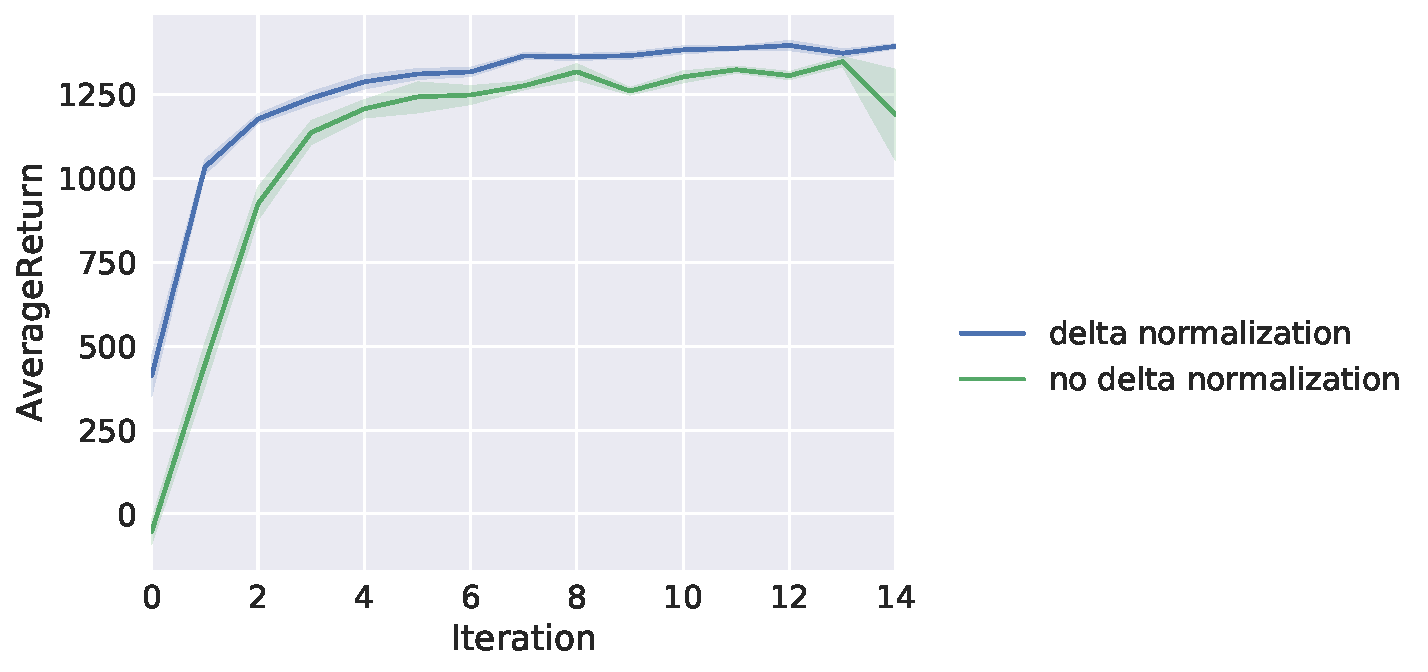
\includegraphics[width=0.8\textwidth]{delta-AverageReturn.pdf}}
  \end{center}
  \caption{Comparison of average returns for on-policy aggregation with a randomly-sampling MPC controller between $\delta$-normalization and no $\delta$-normalization.}
\label{fig:deltanorm}
\end{figure}

Unfortunately, it seems that this intuition is unsuccessful. It seems that normalizing the transitions improves learning. This may be because the transitions themselves $\delta$ have at least a partially stationary distribution (which we might model as a sum of a stationary and a nonstationary component), and normalizing this component still improves learning by keeping the neural network targets at least partially normalized.

\FloatBarrier

\section{Extension: BPTT}

Instead of using expensive MPC rollouts, I considered training a policy to minimize cost directly, back propagating through time (BPTT), through the dynamics that I learned.

In other words, I consider the following explicit, unconstrained minimization, where $\theta$ are our policy parameters, and our dynamics $f$ are fixed and smooth and have known cost $c$:
$$
\argmin_{\theta}\E_{s_0}\sum_{t=0}^H c(s_t,\pi_{\theta}(s_{t}),s_{t+1});\;\;\;\; s_{t+1}\triangleq f(s_t,\pi_\theta(s_t))
$$
Note that the above notation $s_t$ should not be confused with optimization variables---the full expression above is an unconstrained minimization by $\theta$ in terms of $c,f$ alone.

The above computation graph can be expressed in space linear in $H$, so it is tractable to do gradient descent. However, this optimization, as warned in lecture, suffers from several issues. First, we may have the standard RNN issue of vanishing gradients. Second, we may suffer from minor inaccuracies in the dynamics, which may deviate from reality significantly at the end of a simulated rollout but are incorporated in the optimization of $\theta$. I attempted solve these issues by (1) using a gated recurrent unit (GRU) as the policy architecture and (2) reducing $H$ from the full $1000$ to $50$ and sampling the initial state $s_0$ from the on-policy state distribution (so the policy trains on random segments within an episode).

Nonetheless, the results were still pretty bad, but it was cool to find out that BPTT really does suck when combined with a shooter method from learned dynamics. ,  the training task (Fig.~\ref{fig:bptt}). Notably, test-time performance is an order of magnitude faster (since we have no rollouts to simulate). We still need to train the policy instead now, but total iteration time is reduced to \textbf{${\mathbf{23.74
}}$ seconds}.

\begin{figure}[!h]
  \begin{center}
    {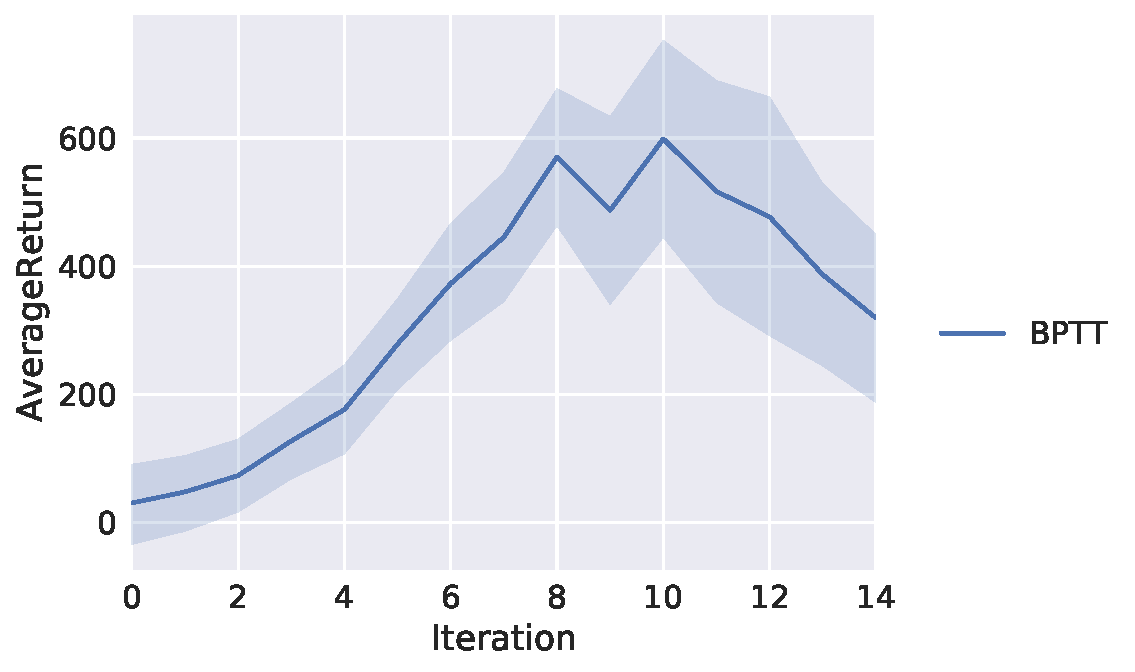
\includegraphics[width=0.8\textwidth]{bptt-AverageReturn.pdf}}
  \end{center}
  \caption{Average return over policy aggregation iterations for the BPTT agent. I use 2 stacked GRU units with 32 hidden units each for the BPTT policy with a learning rate of $10^{-5}$, a mini-batch size of 512, and 1 epoch of training per on-policy iteration.} 
\label{fig:bptt}
\end{figure}

I tried stacked RNN units up to 5 stacked GRUs over variable sizes 8, 16, 32, each over different learning rates $10^{-5},10^{-4},10^{-3}$, with variable simulation horizons (15, 50, 100), epochs of training (1, 10, 100), and batch sizes (64, 512, 8196). Everything looked as noisy/bad as Fig.~\ref{fig:bptt}. I figure that this is the case even with a GRU policy because the GRU policy accepts the states as inputs, but states are not independent data---they're generated by the frozen dynamics $f$, which is a function of the actions generated by the policy. Perhaps gradients are exploding through this path of the computation graph (and, if so, then perhaps we can make the dynamics $f$ a GRU as well)?

\FloatBarrier

\section{Extension: Smarter Sampling}\label{smart-sample}

Instead of random sampling, one might attempt to have a more intelligent MPC rollout. In particular, we can have a policy learn the from the MPC expert: every iteration we train a neural network from our aggregated policy to mimic the MPC rollout. Then, when we sample, we use MPC control, but only with the first action randomly sampled at uniform. All then next actions are taken by the learned policy. By having more reasonable simulated rollouts, MPC can choose smarter initial actions. The neural network training wasn't a noticeable additional time cost, but resulted in much-improved performance (Fig.~\ref{fig:mpcmf}).

\begin{figure}[!h]
  \begin{center}
    {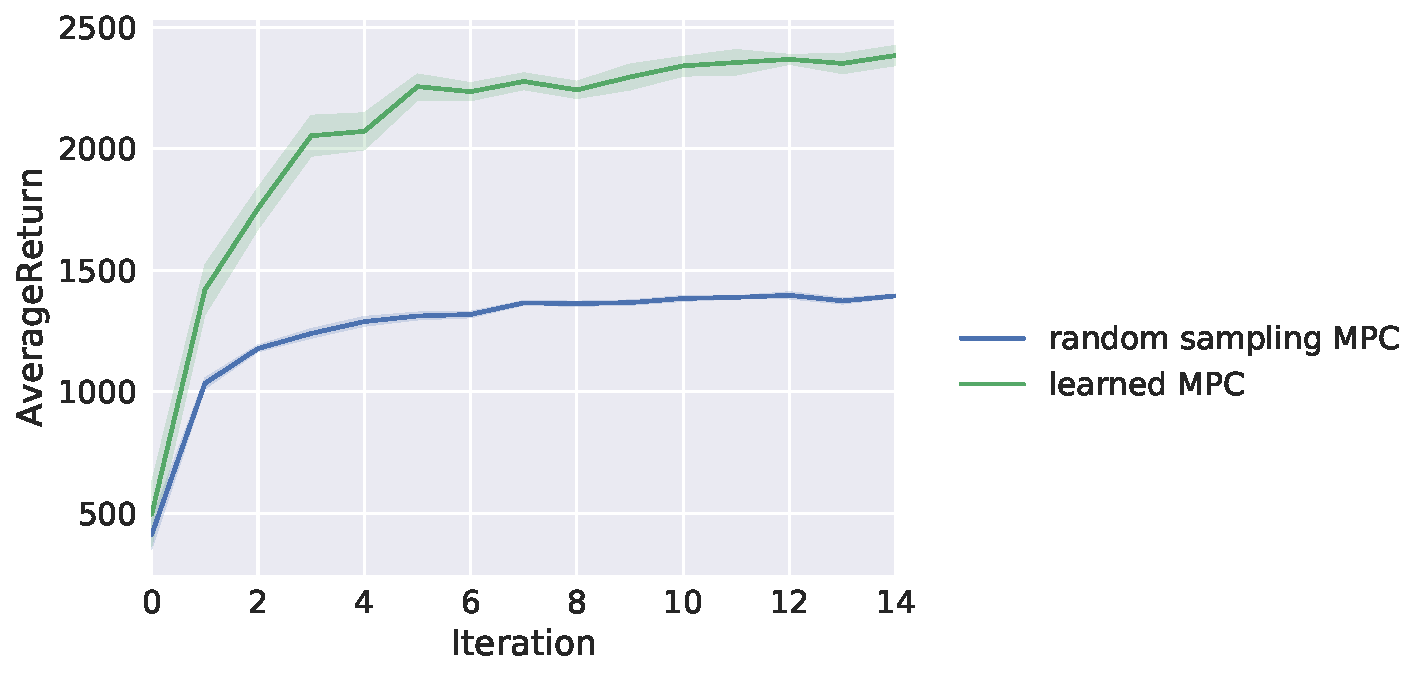
\includegraphics[width=0.8\textwidth]{mpcmf-AverageReturn.pdf}}
  \end{center}
  \caption{Average return over policy aggregation iterations for the learning-based sampling MPC agent, compared to the standard uniform sampling MPC agent.}
\label{fig:mpcmf}
\end{figure}

This results in a pretty interesting ``bootstrapping'' effect where the MPC expert gets better by relying on what is essentially a memoized version of itself. Note that the learner neural network is only used starting on the second step of the MPC rollout simulations, with the first one still randomly sampled. This strategy seems pretty similar to MCTS, but in a continuous setting (where we have a policy picking the action to take).

\FloatBarrier

\section{Conclusion}

I expect that it may be possible to speed up test-time execution by using the learned policy network mentioned in Sec.~\ref{smart-sample}, with a DAGGER-style approach as mentioned in the paper: use the learned policy network to make sampling decisions, and only rely on the MPC controller (perhaps using the policy network for sampling again) for expert annotations. When I tried this, I found that the policy network did not have variable-enough performance to explore sufficiently. Perhaps this was just a matter of messing with variance hyperparameters for the learned network's Gaussian policy, but I tried quite a few. I noticed that the paper mentioned in the assignment warm-started the dataset with (randomly-sampled) MPC samples (whereas I did a cold-start from training on expert-labelled states generated by the random agent). Perhaps the warm-start was key, but it feels like cheating, since you need to run your MPC samples anyway.

\end{document}
